\section{Ethereum Core Components}\label{ethereum-core-components}

\subsection{Network}\label{network}

The underlying network that Ethereum is built on is a peer-to-peer
network that's nowadays running on TCP port 30303. The protocol that
enables this P2P network is known as Ð$\Xi$Vp2p.

If you step back and think about the paradigm of the networks that we
use today is built around the concept of clients and servers: Laptops,
desktops, smartphones, iot gadgets\ldots, that we use are all really the
clients that are talking to servers sitting in the cloud on AWS or any
of the application platforms that you're interacting with.

Compared to that, the key change when it comes to Ethereum is that
\textbf{the underlying network is all peer-to-peer}: there are no
clients and servers, they're all peers that are exchanging messages on a
same layer.

On this network we have transactions, which imply the notion of a sender
transferring some value (and some data) to a receiving entity.

And on top of that there is this abstraction of a state machine that is
driven by the EVM. When it comes to programming that machine, there are
high-level languages (HLLs) that programmers and developers work with,
being the most common one (the most widely used) \texttt{Solidity},
which is converted into EVM instructions (machine language instructions;
bytecode).

\subsection{Data Structures}\label{data-structures}

The Ethereum protocol itself has several common data structures. There
is however a very specific data structure known as the
\textbf{Merkle-Patricia Tree} that is used to optimize the way that
Ethereum handles some of the states that are used within the context of
the blockchain.

\begin{itemize}
\item
  \textbf{Merkle Tree}

  A Merkle Tree is a type of binary tree that is composed of a set of
  nodes where the leaf node at the bottom of the contains the underlying
  data, and all the intermediate nodes between the leaf nodes and the
  root contain the combined hash of their two child nodes. Visually, the
  data is located at the bottom of the leaf nodes, and all the
  intermediate nodes (combining their hashes) lead to the root node,
  which is at the top of the tree and it's usually referred to as
  ``\emph{the root hash}''.

  \begin{figure}
  \centering
  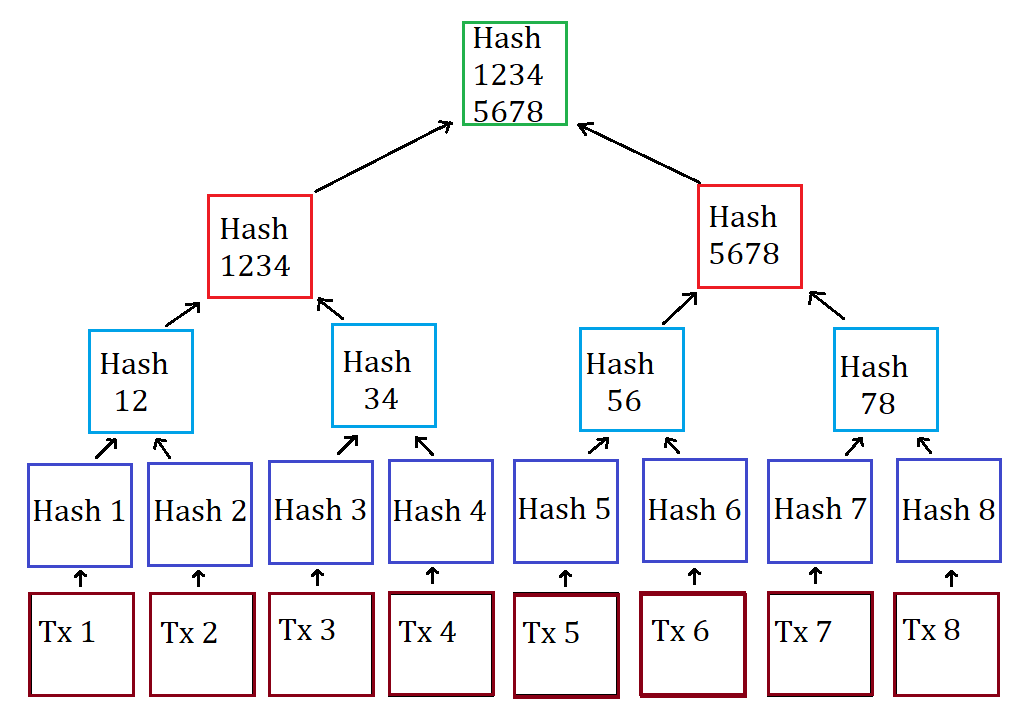
\includegraphics[width=\linewidth]{../src/img/Merkle_Tree.png}
  \caption{Merkle Tree example consisting of 8 underlying transactions.}
  \end{figure}
\item
  \textbf{Patricia Tree}

  A Patricia tree (aka prefix free radix tree) is a different data
  structure where the \texttt{(key,\ value)} pairs that are contained
  within it have the values at the leaf nodes, and the keys let you
  traverse a path from the root of the tree to the leaves, so that the
  nodes that share the same prefix in the key also share the same path
  down the tree from the root to the leaves.

  \begin{figure}
  \centering
  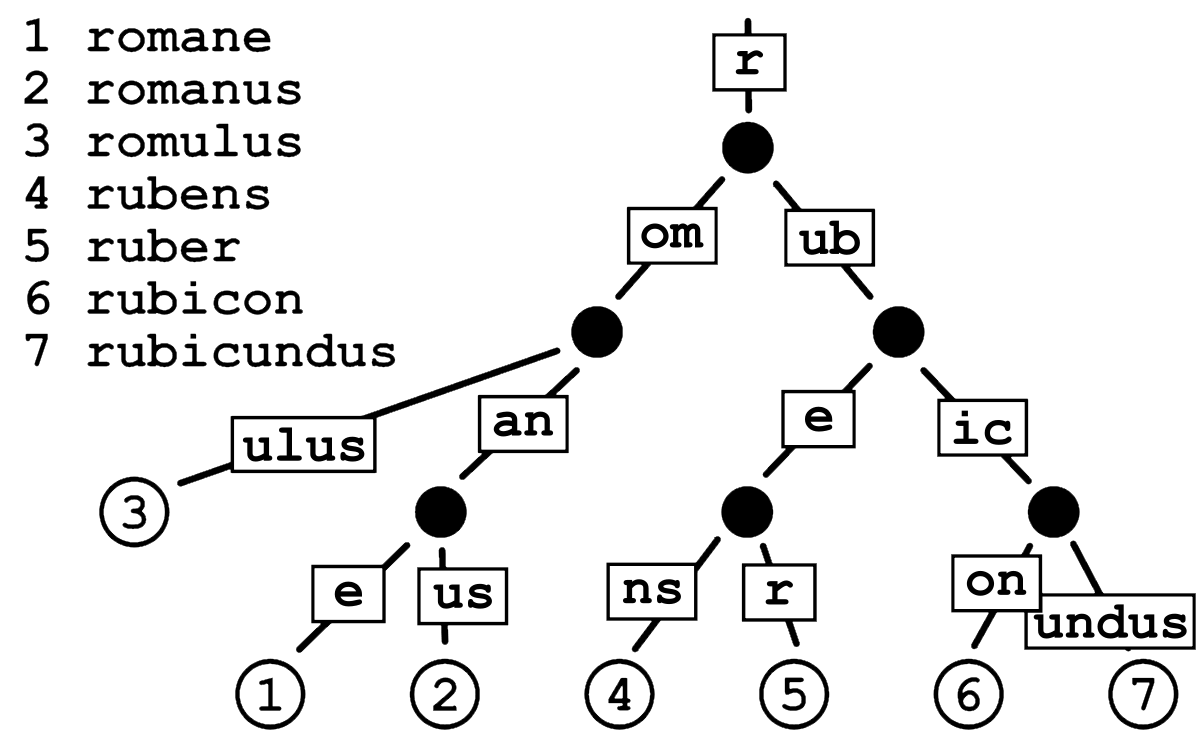
\includegraphics[width=\linewidth]{../src/img/Patricia_Tree.png}
  \caption{Patricia Tree Example}
  \end{figure}

  Ethereum uses a modified combination of a Merkle tree and Patricia
  tree that specifically suits the Ethereum data structures. In this
  particular case, it uses a Hexane-Merkel-Patricia tree which means
  that each node has 16 children. There's also a recent proposal to
  convert this to a binary tree.
\item
  \textbf{Other data structures}

  When looking at the programming languages supported on Ethereum, let's
  take for example \texttt{Solidity}, there are many common data
  structures such as arrays, lists, the basic value types, reference
  types\ldots{}
\end{itemize}

\subsection{Consensus Algorithm}\label{consensus-algorithm}

One of the critical core compontents (perhaps the most critical one) is
the consensus algorithm.

\begin{itemize}
\item
  \textbf{Why is there a need for a consensus algorithm this?}

  The Ethereum blockchain, as mentioned earlier, consists in many
  peer-to-peer nodes: these nodes are all talking to each other and
  trying to agree upon what is the global state of the blockchain.\\

  Each of the nodes has a local state, which consits on new blocks being
  formed containing the transactions that are processed by the node. But
  then, everyone on the Ethereum blockchain should agree upon what is
  the one canonical blockchain that will be used in the future.\\

  This is agreement is reached through the \textbf{consensus algorithm}.
  Decentralized consensus is critical to any blockchain. In the context
  of Ethereum it refers to the \textbf{Nakamoto Consensus Protocol} that
  is adapted from Bitcoin. This protocol addresses the problem of which
  miners' block should be included next to create the canonical
  blockchain. There are two components to this: \textbf{Proof of Work}
  (PoW) and \textbf{The longest chain rule}.\\

  PoW is used to determine which entity on the Ethereum blockchain gets
  to add the next block; \textbf{the consensus algorithm} determines
  which is the longest chain so far, and all the nodes that are chosen
  to add the next block to the existing canonical blockchain build upon
  the existing longest chain. This is how a blockchain grows in state.\\

  The consensus algorithm is used as a form of \textbf{sybil resistance}
  mechanism. There's this concept of 51\% attack, which consists in the
  scenario of 51\% of the participating entities colluding. Then, these
  malicious entities can change past states (and thus the state
  transitions) that have been encoded into the blockchain. This breaks
  the key property of immutability of a blockchain, thus it is very
  critical.
\end{itemize}

\subsection{Ethereum PoW: Present and
Future}\label{ethereum-pow-present-and-future}

As mentioned previously, Ethereum Proof of Work is fundamental to how
the Ethereum consensus protocol works. Technically, it is referred to as
Ethash, and it's formally defined as

\begin{align*}
(m,n)&=\text{PoW}\left(H_{\stkout{n}},H_n,d\right)\\ m&=H_m\wedge n\leq\frac{2^{256}}{H_d}
\end{align*}

where $H_\stkout{n}$ is the new block's header but without the nonce ($n$)
and mix-hash ($m$) components; $H_n$ is the nonce of the header;
$d$ is a large data set needed to compute the mixHash and $H_d$ is
the new block's difficulty value.

What a miner has to do is to determine a combination of mix-hash $m$
and nonce $n$ for every block to satisfy the constraint on the
difficulty for that particular block. This is a trial and error process
so the miner has to keep repeating the computation until a combination
of $m$ and $n$ that satisfies the difficulty is found. When this is
done it means that a sufficient amount of work has been performed by the
miner for this particular block, or in other words this indicates that
there is proof of work by the miner for this block.

PoW is being replaced by what is known as \textbf{proof of stake} (PoS)
with \textbf{the merge}. This change is important from a security
perspective: the consensus algorithm is critical to the economic
security of a blockchain, as it is what makes the blockchain resistant
to attacks from any of the untrusted parties operating the
infrastructure or operating on it. For now, this security is provided by
PoW.

\subsection{\texorpdfstring{Ethereum protocol upgrades (initially
\texttt{Eth2})}{Ethereum protocol upgrades (initially Eth2)}}\label{ethereum-protocol-upgrades-initially-eth2}

\textbf{The merge} the first of a set of interconnected upgrades to the
existing Ethereum network that are being made, perhaps the biggest set
of upgrades since Ethereum started. Although it was initially coined as
\texttt{Eth2}, this name was phased out because it is not a separate
version of the protocol but a continuation of all the research and
development activity that has happened on the protocol. These upgrades
occur across three vectors: \textbf{scalability}, \textbf{security} and
\textbf{sustainability}.

\begin{itemize}
\item
  \textbf{Scalability}: made possible by the concept of sharding.\\
\item
  \textbf{Security}: through the transition from PoW to proof of stake
  (PoS), also known as the merge.

  This is again a huge change to how the protocol functions and it
  offers immense economic and security benefits compared to PoW.\\
\item
  \textbf{Sustainability}: with PoW, there's a certain amount of
  computation that has to be done to pass the difficulty level. This is
  for sybil resistance part of the consensus protocol.\\

  As a result, there is real energy (in terms of running the mining
  nodes) that is consumed. This goes away to a great extent when we
  transition to PoS: it is going to make Ethereum much more sustainable
  when it comes to environmental impact.
\end{itemize}

These upgrades already started happening with the deployment of the
Beacon chain and the transition to PoS with the merge.

\subsection{Ethereum Nodes and
Clients}\label{ethereum-nodes-and-clients}

An Ethereum node is a software application that implements the Ethereum
protocol specification. It communicates with other Ethereum nodes on the
network in a peer-to-peer fashion.

The Ethereum client is a specific implementation of the Ethereum Node.
Within the Ethereum clients, a specification of the protocol itself (the
consensus algorithms, data structures,\dots all these core components)
is implemented.

If anyone is running an Ethereum node they're using one of these
Ethereum clients that have been built by multiple teams around the
world. The most popular ones are

\begin{itemize}
\tightlist
\item
  Geth
\item
  Erigon
\item
  Nethermind
\item
  OpenEthereum
\item
  Reth
\end{itemize}

There have been a lot of transitions and changes. Some of the clients
have been under development, and some of them are way more popular. Geth
is the most popular with more than 80\% of the running nodes. But, for
the sake of the diversity and decentralization of Ethereum, other
clients are being supported and being developed as well. These clients
are open source so anyone is free to examine the client code and maybe
even contribute to it.

Ethereum transactions are sent to the Ethereum Nodes, and these in turn
broadcast them across the peer-to-peer network. This is how Ethereum
transactions propagate across the Ethereum network, reach the various
nodes, get combined into blocks and result in the blockchain.

\subsection{Ethereum Miners}\label{ethereum-miners}

Ethereum miners are entities running Ethereum Nodes on the network. They
are the ones that receive, validate, execute and combine the
transactions into blocks.

They also provide a mathematical proof of their computation (proof of
work; PoW). For all this work, if the miner's block gets chosen to be
part of the blockchain, then they are rewarded with what is known as a
block reward.

This block reward is currently 2 Ether and it has decreased over time.
This is the crypto economics: incentive for miners to participate and to
be honest on the Ethereum network. Along with this reward, they're also
rewarded with transaction fees: the Ether spent on Gas by all the
transactions included in that block.

So block reward and transaction fees are the crypto economic incentives
that are paid out to the miner whose block gets accepted into the
blockchain.

\subsection{GHOST protocol}\label{ghost-protocol}

So transactions are sent, and miners validate them. They combine them
into blocks and these blocks are propagated over the peer-to-peer
network. Multiple miners are doing this process simultaneously. This
leads to multiple valid blocks at any level of the blockchain. The
canonical blockchain needs to choose one valid block at any level. The
choice of that valid block is dictated by the ``\emph{\textbf{GHOST
protocol}}'' (the Greedy Heaviest Observed Subtree protocol). This
protocol allows stale blocks up to seven levels in this calculation.
Stale blocks, in Ethereum's nomenclature, are referred to as uncles or
armors.
